\documentclass[a4paper,10pt]{article} % Changer la taille de police c'est ici

\usepackage{framed} % Marges
\usepackage[utf8]{inputenc} %francais
\usepackage[T1]{fontenc} %francais
\usepackage[french]{babel}  %francais
\usepackage{lmodern} % Pour changer le pack de police
\usepackage{makeidx} % Index
\usepackage{graphicx} % Figures
\usepackage{wrapfig} % Figures
\usepackage{amsmath} % Maths
\usepackage{amssymb} % symboles ?
\usepackage{bclogo} % ?????
\usepackage{stmaryrd}
\usepackage[top=2cm, bottom=2cm, left=2.5cm, right=2.5cm]{geometry} %Marges

\renewcommand{\baselinestretch}{1.3} %Interligne

\title{\textbf{Interpolaspline}}
\author{Rapport du stage applicatif\\ L3 MIN}
\date{\emph{Décembre 2019}\\CORBILLE Clément, DOUMBOUYA Mohamed, EL BOUCHOUARI Zakaria, HEDDIA Bilel, PIASENTIN Béryl, RODET Amélys}

\begin{document} %Ne rien ecrire avant

\maketitle % titres
\tableofcontents %Tables des matieres

\newpage

\section*{Introduction}
\addcontentsline{toc}{section}{Introduction}
Dans le cadre de notre troisième année de licence mathématiques-informatique à l’Université Grenoble Alpes, nous devons effectuer un stage applicatif à l’UFR IM$^2$AG. Ce stage, qui consiste en un projet, est une étape indispensable pour mettre en pratique les connaissances acquises durant cette formation et pour acquérir de nouvelles compétences de recherche. Les projets ont lieu durant quatre semaines, réparties en deux périodes de respectivement une puis trois semaines. Des groupes de six étudiants ont été construits en fonction des affinités de chacun pour les différents sujets proposés.

Le sujet de notre projet est l'interpolation avec données aberrantes. Il nous donne l’opportunité d’approfondir nos connaissance en Mathématiques appliquées, plus précisément d'approfondir l'enseignement d'algèbre linéaire pour le graphique et la CAO (Conception Assistée par Ordinateur) que nous avons reçu, ainsi que la programmation en langage  python. De plus, ce stage va nous permettre d'acquérir des compétences en travail de groupe.

\section{Organisation de la semaine}

L'objectif de cette semaine de stage était de mettre en place l'organisation nécessaire à la réalisation du projet qui aura lieu en avril.

Nous avons commencé par désigner un chef de projet : Béryl a été choisie à cet effet. La chef de projet veille sur le bon déroulement de chaque tâche en plus de sa participation aux différentes tâches. Nous avons ensuite défini un nom pour le projet, en rapport avec le contenu mais également percutant. "Interpolaspline" a été le nom retenu, en tant que fusion du mot "interpolation" et du mot "spline", deux notions principales du sujet.

Durant cette semaine d'organisation, chaque membre du groupe a été responsable d’une ou de plusieurs tâches. Etre responsable d'une tâche signifie s'assurer que celle-ci est correctement réalisée et terminée dans les délais fixés, mais pas obligatoirement qu'elle doit être réalisée seul.

Les premiers jours ont été mis à profit pour comprendre le sujet et trouver ce sur quoi nous allions travailler pendant trois semaines. Il a fallu ensuite établir un plan de travail. Cette reflexion nous a permis de construire un diagramme de Gantt et un graphe de dépendances des tâches, mais aussi de répartir les tâches entre les différents membres du groupe. Chacun sait donc de quelle tâche il est responsable et peut se projeter dans la semaine de réalisation.

Une fois tous ces points mis en place, nous avons établi le cahier de charges. Nous y avons décrit le problème, nos objectifs, le cadre du projet. La description des fonctionnalités livrées à la fin du projet y est également détaillée, ainsi que l'organisation temporelle du projet. 

Tous les membres du groupes ont participé à la rédaction du rapport basé sur cette semaine de travail, incluant le cahier des charges, mais aussi à la préparation de la soutenance. Pour terminer cette semaine d'organisation, chacun a pris le temps de bien comprendre ce qu'il devrait faire durant les trois semaines de réalisation. 
\newpage
\section{Contexte et objectifs}
	REDIGER DU BLABLA SUR QQOQCCP

\section{Définition des tâches}

	\subsection{Création des tâches}
	Dans le but d'interpoler des données en utilisant des splines de lissage tenant compte des valeurs aberrantes, nous nous devions de savoir comment aborder le sujet. En discutant entre membres du groupe, nous avons convenu qu'il fallait dans un premier temps approfondir les notions générales sur les splines naturelles et de lissage en fonction de la répartition des points et trouver un moyen d'automatiser l'estimation du paramètre de lissage. Puis nous avons prévu d'étudier des méthodes d'identification des valeurs aberrantes que l'on souhaite à terme implémenter en deux dimensions, mais aussi des méthodes permettant d'interpoler des splines sans commencer par détecter les valeurs aberrantes.
\newpage
	\subsection{Contenu des tâches}
	Les tâches sont les suivantes :
\begin{itemize}
\item Approfondissement des splines naturelles
\item Approfondissement des splines de lissage uniformes
\item Approfondissement des splines de lissages non-uniformes
\item Estimation automatique du paramètre de lissage
\item Identification des points aberrants
\item Etude des splines de lissage avec points aberrants
\item Etude de l'algorithme RANSAC
\item Redéfinition d'autres fonctions d'erreur à minimiser
\item Finalisation du projet
\end{itemize}

Voici quelques explications du contenu scientifique constituant la base des tâches listées ci-dessus.
\subsubsection*{Splines naturelles}
L’interpolation est une opération mathématique consistant à déterminer une fonction passant par un nombre fini de points donnés.

Soient $(x_i,y_i)$ les $n+1$ données, $i\in\llbracket 0; n \rrbracket$.
Une spline est une fonction définie par morceaux sur chaque intervalle $[x_i, x_{i+1}]$, $i\in\llbracket 0; n-1 \rrbracket$.
Le principe d'une spline est de combiner plusieurs morceaux de fonctions (en général on utilise des polynômes de petit degré) pour former une fonction d'une classe définie.

Les splines cubiques $C^2$ sont les splines définies par des polynômes cubiques dont la dérivée seconde est continue. On appelle spline naturelle la spline cubique $C^2$ dont les dérivées secondes aux extrémités de l'intervalle de définition sont nulles. La spline naturelle existe toujours pour des données distinctes, et est unique. Le principe de la spline cubique naturelle permet d'obtenir un système tridiagonal simple qui peut être résolu facilement, afin d'obtenir les coefficients des polynômes.

\subsubsection*{Splines de lissage}
Les splines de lissage sont des splines cubiques naturelles dont chaque polynôme cubique est une approximation des données se trouvant sur son intervalle de définition. Cette spline ne passera dans la plupart des cas pas par tous les points, mais est la spline qui minimise une quantité liée à la distance entre les données et la spline. En général, la spline approximant les données cherche à minimiser l'erreur au carré : c'est l'approximation aux moindres carrés. 
Les splines de lissage permettent d'éviter les oscillations qui seraient présentes avec une spline naturelle passant par tous les points, provoquées avec un nombre de données très grand.

\subsubsection*{Paramètre de lissage}
La quantité à minimiser pour construire la spline approximant des données est composée de deux parties dont la seconde est pondérée par un paramètre de lissage : la première assure le passage de la spline par nos données tandis que la seconde assure le lissage de la courbe. Cela signifie que plus on augmente la valeur du paramètre de lissage, plus le lissage sera fort ce qui donne par suite une spline passant de moins en moins proche des données.

\subsubsection*{Données aberrantes}

En statistiques, une donnée aberrante est une valeur ou une observation qui est « distante » des autres observations effectuées sur le même phénomène, c'est-à-dire que c’est une valeur qui s'écarte fortement des valeurs des autres observation : elle est anormalement faible ou élevée par rapport à celles qui lui sont proches. Sur un graphe on peut les visualiser comme des points qui se situent loin du nuage de points principal.

Les  méthodes pour créer une spline de lissage malgré les données aberrantes sont variées : certaines déterminent les points aberrants pour ensuite les supprimer ou leur associer un poids faible tandis que d'autres créent la spline tout en gérant les points aberrants, sans les détecter auparavant. 

\subsubsection*{RANSAC}

RANSAC est l'abréviation de RANdom SAmple Consensus, c'est à dire consensus d'échantillons aléatoires. C'est le nom d'un algorithme qui gère les points aberrants sans prendre le temps de les détecter dans un premier temps. Cet algorithme est itératif, et non-déterministe. Un algorithme non déterministe est un algorithme qui ne produit pas toujours la même sortie pour une même entrée.

\subsubsection*{Interpolation paramétrique}

L'objectif de l'interpolation paramétrique est de trouver un polynôme paramétrique qui interpole les données. Pour ce faire, deux méthodes sont possibles :
\begin{itemize}
\item L'interpolation séparée des $n$ données $(t_i,x_i)$ et des $n$ données $(t_i,y_i)$, $i\in\llbracket 0; n \rrbracket$, avec t un paramètre bien choisi. On obtient deux splines P et Q interpolant respectivement les données $(t_i,x_i)$ et $(t_i,y_i)$,$i\in\llbracket 0; n \rrbracket$. En associant les deux splines obtenues grâce au paramètre t, on obtient une spline paramétrique S interpolant les données de départ, $S(t) = (Q(t),R(t))$. En particulier, $P(t_i) = (x_i,y_i)$, $i\in\llbracket 0; n \rrbracket$.
\item L'interpolation en une fois des données, sans appliquer la méthode à une dimension sur chaque dimension.
\end{itemize}


\section{Cahier des charges}

Le cahier des charges est l'annexe n\degre4. Nous y avons détaillé le projet, du sujet à l'archive rendue, en passant par sa réalisation. Ce cahier des charges représente notre compréhension globale du sujet ainsi que les principales idées d'organisation et de réalisation.

Ce document est censé être le lien entre notre équipe et le client, mais il est ici le lien entre notre équipe et l'équipe d'enseignants responsables du stage applicatif. Nous allons l'utiliser durant la seconde fin du projet. Notre objectif est de réaliser tous les objectifs qui y sont définis, dans les délais impartis.

\section{Planification des tâches}

	\subsection{Organisation des tâches}

	\subsection{Répartition des tâches}

\section{Risques}

Le risque majeur du projet est de ne pas avoir estimé correctement le temps necessaire pour réaliser certaines tâches. En effet, si une fonctionnalité met trop de temps à être implémentée, certaines tâches qui en dépendent risquent de prendre du retard, cela est l'effet boule de neige. Pour éviter cela, le diagramme de Gantt prévoit des membres "flottants", qui se greffent sur les tâches posant des difficultés.

\section*{Conclusion}
\addcontentsline{toc}{section}{Conclusion}

Lors de cette semaine travail nous avons remarqué qu‘au final, nous avons eu une bonne cohésion de groupe. Etant donné qu’au début du projet nous avons tous des idées différentes, nous avons toutefois réussi à nous mettre d’accord sur une trame de projet. Cette cohésion n’était pourtant pas évidente lors de la formation de notre groupe puisque les groupe sont formé en fonction des sujets. Afin de suivre cette tram, nous avons donc dû organiser. C’est-à-dire que nous avons partagé le travail en groupe en sorte que chacun ait au moins une tâche, afin de gagner du temps. Nous nous sommes même découvert une âme d’acteur pour chacun d’entre nous, c’est pourquoi selon les caractères et personnalités de chacun nous avons attribué les rôles afin que cela soit le plus cohérent possible.

\section*{Annexes}
\addcontentsline{toc}{section}{Annexes}

\begin{itemize}
\item[1.] Diagramme de Gantt (partie 1)
\item[2.] Diagramme de Gantt (partie 2)
\item[3.] Diagramme de Gantt simplifié et répartition des tâches
\item[4.] Graphe de dépendance des tâches
\item[5.] Cahier des charges
\end{itemize}
\begin{figure}
\begin{center}
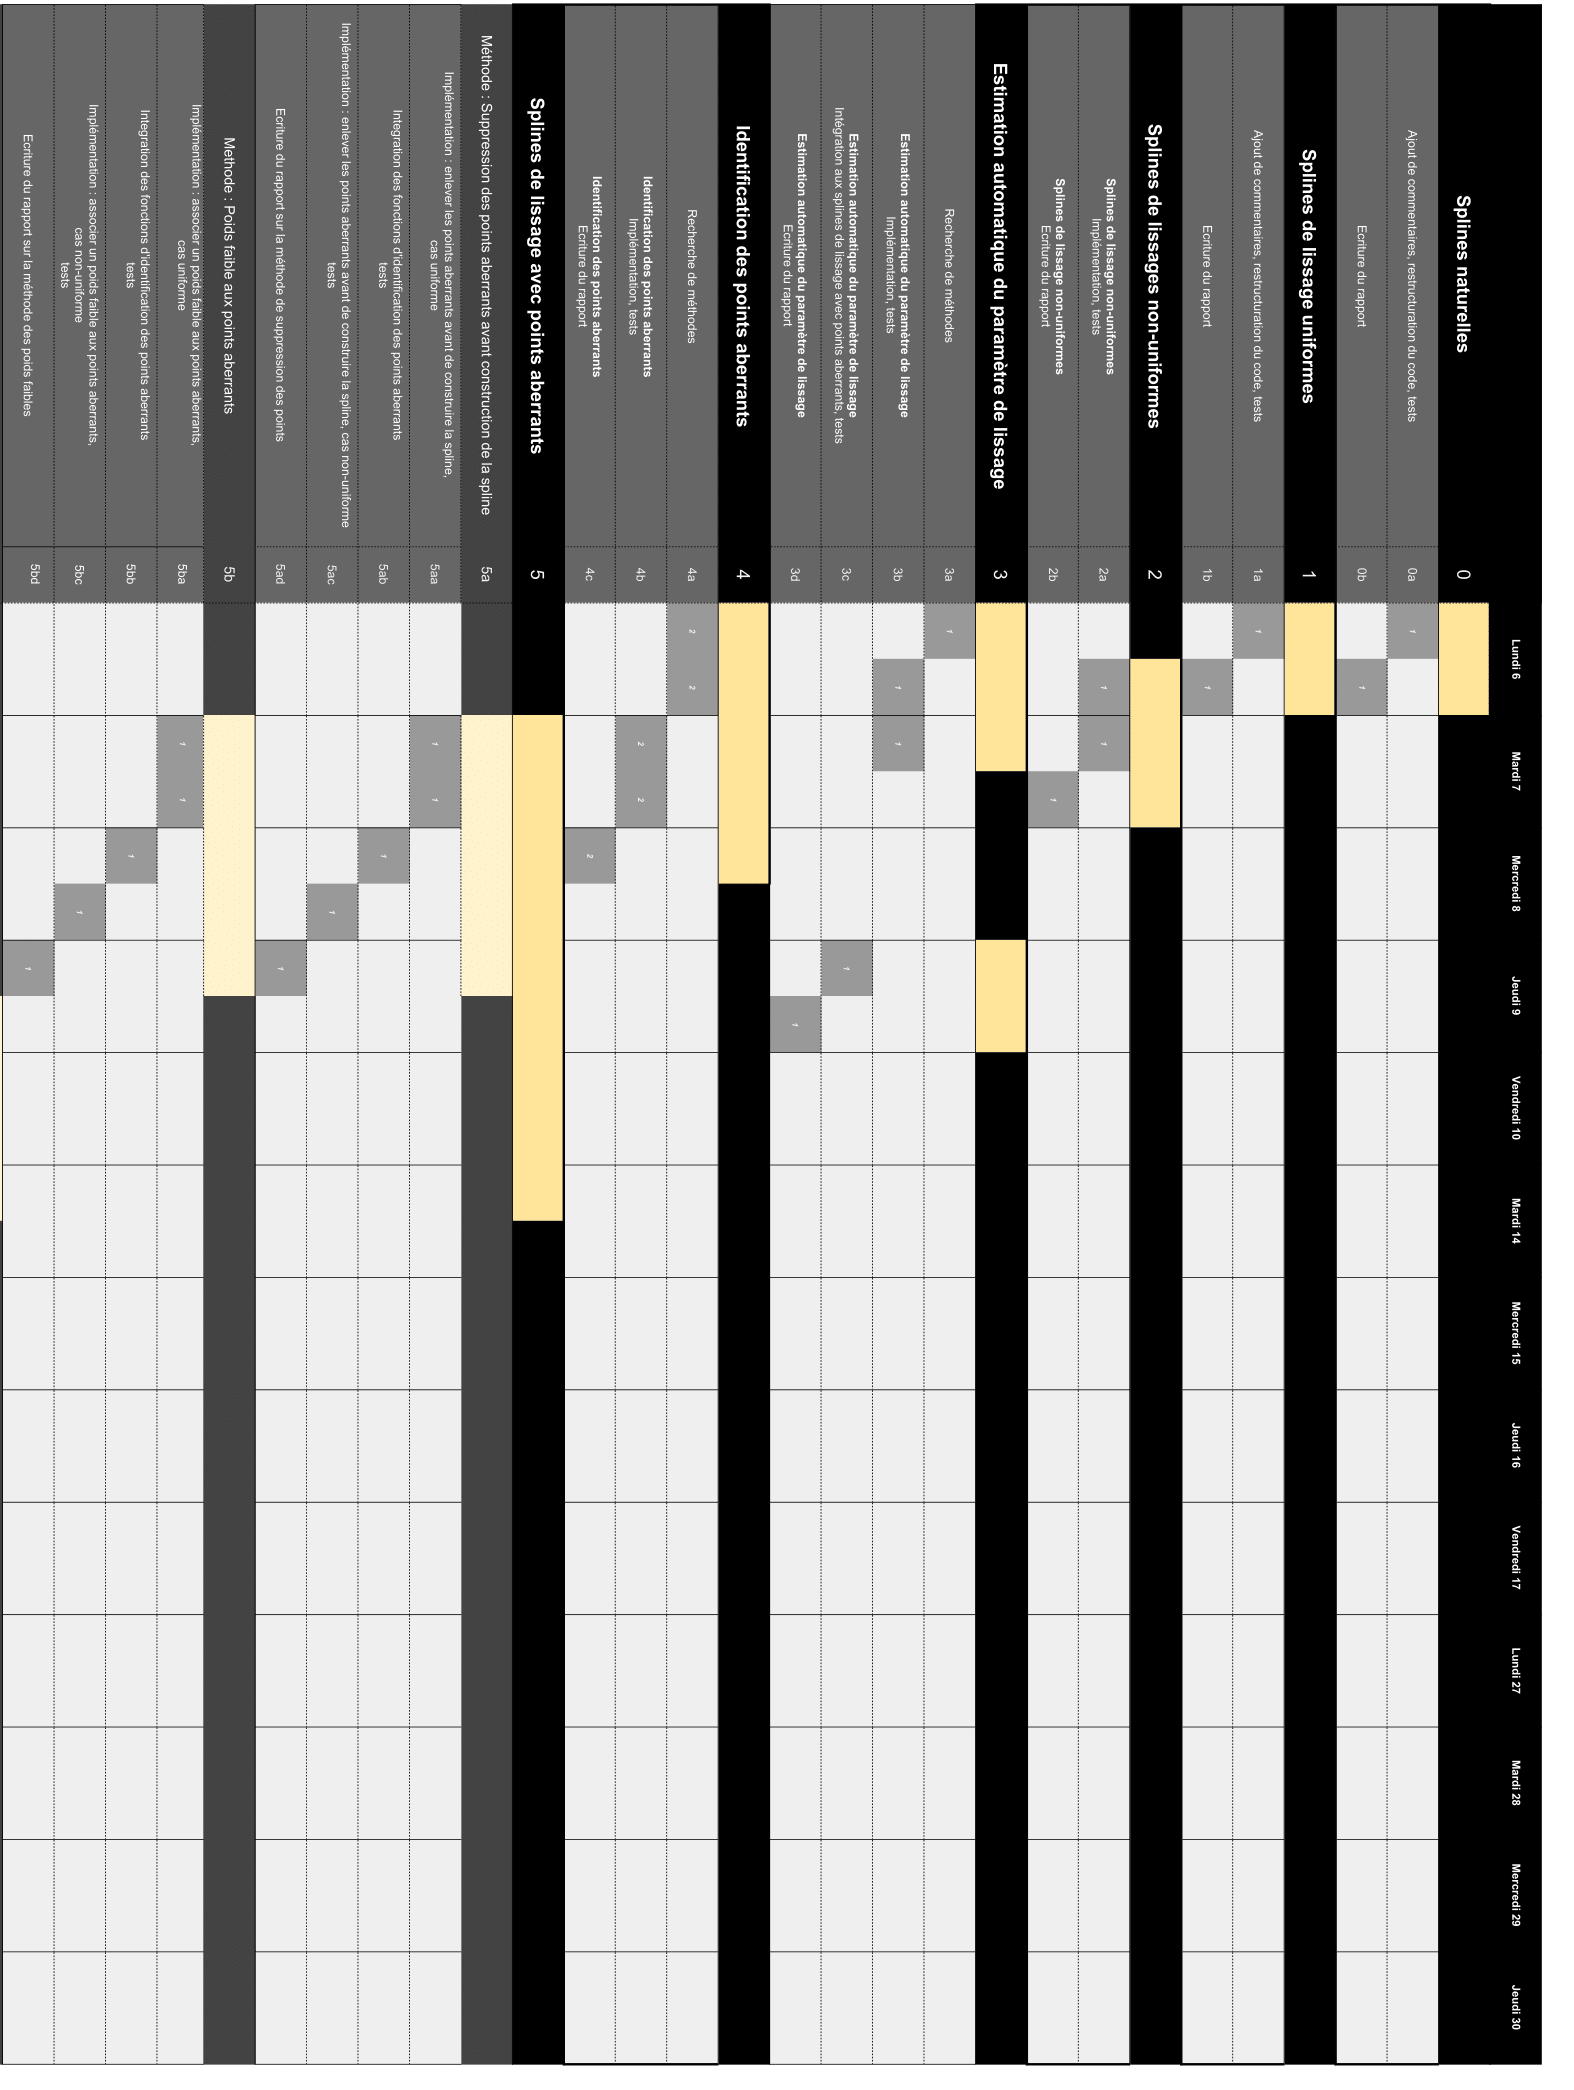
\includegraphics[width=16cm]{p1.png} 
\end{center}
\caption{Diagramme de Gantt (partie 1)}
\label{DiagG1}
\end{figure}

\begin{figure}
\begin{center}
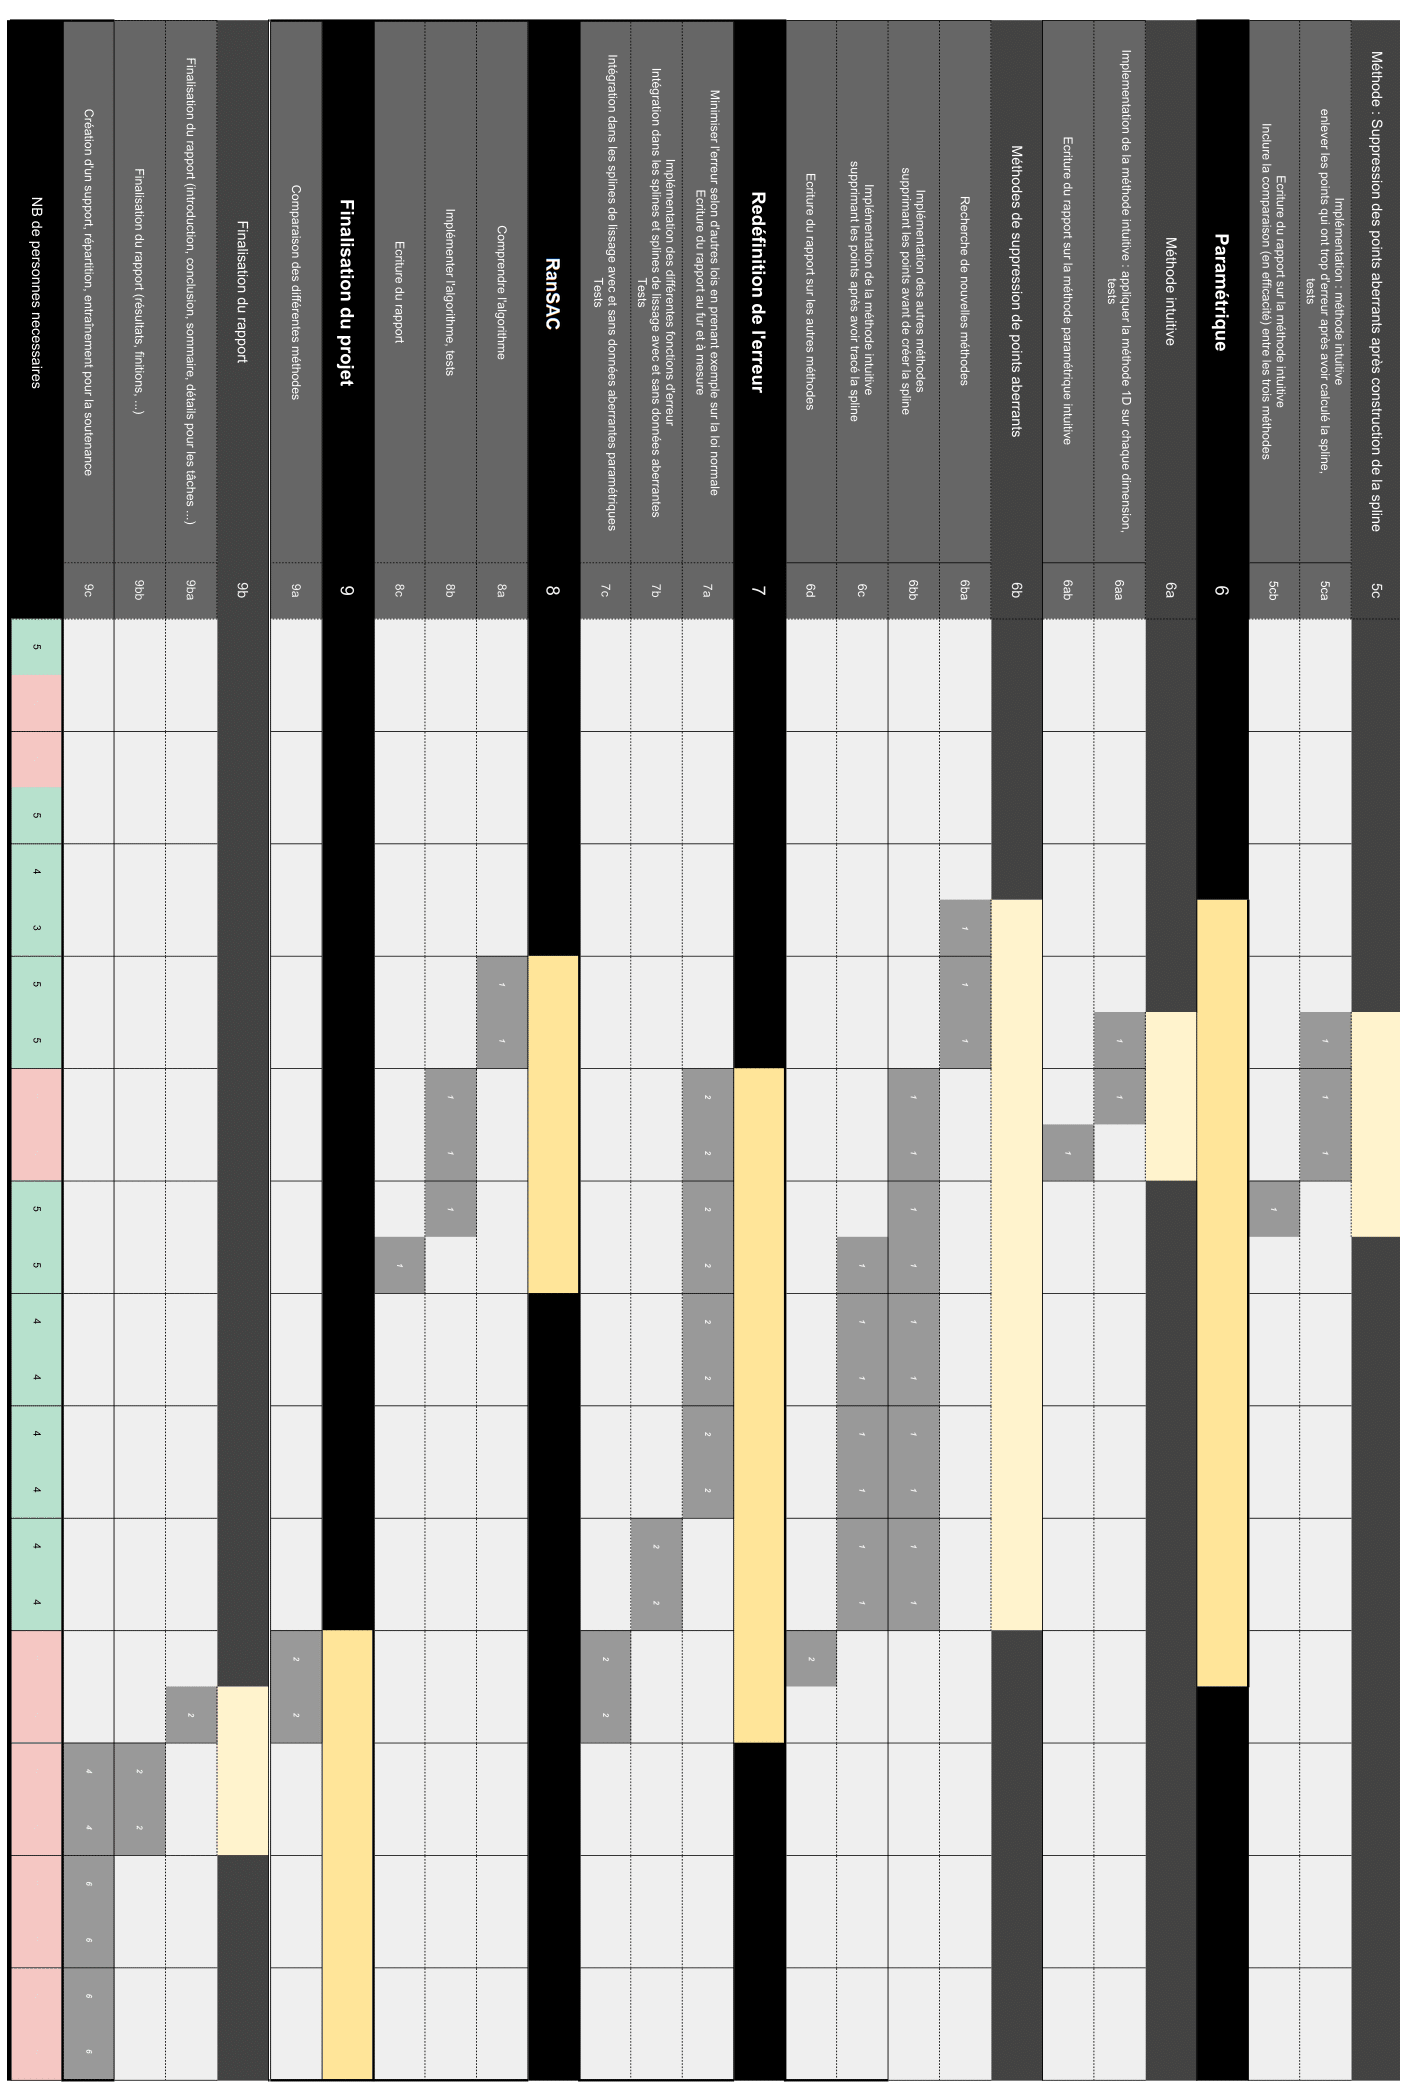
\includegraphics[width=16cm]{p2.png} 
\end{center}
\caption{Diagramme de Gantt (partie 2)}
\label{DiagG2}
\end{figure}

\begin{figure}
\begin{center}
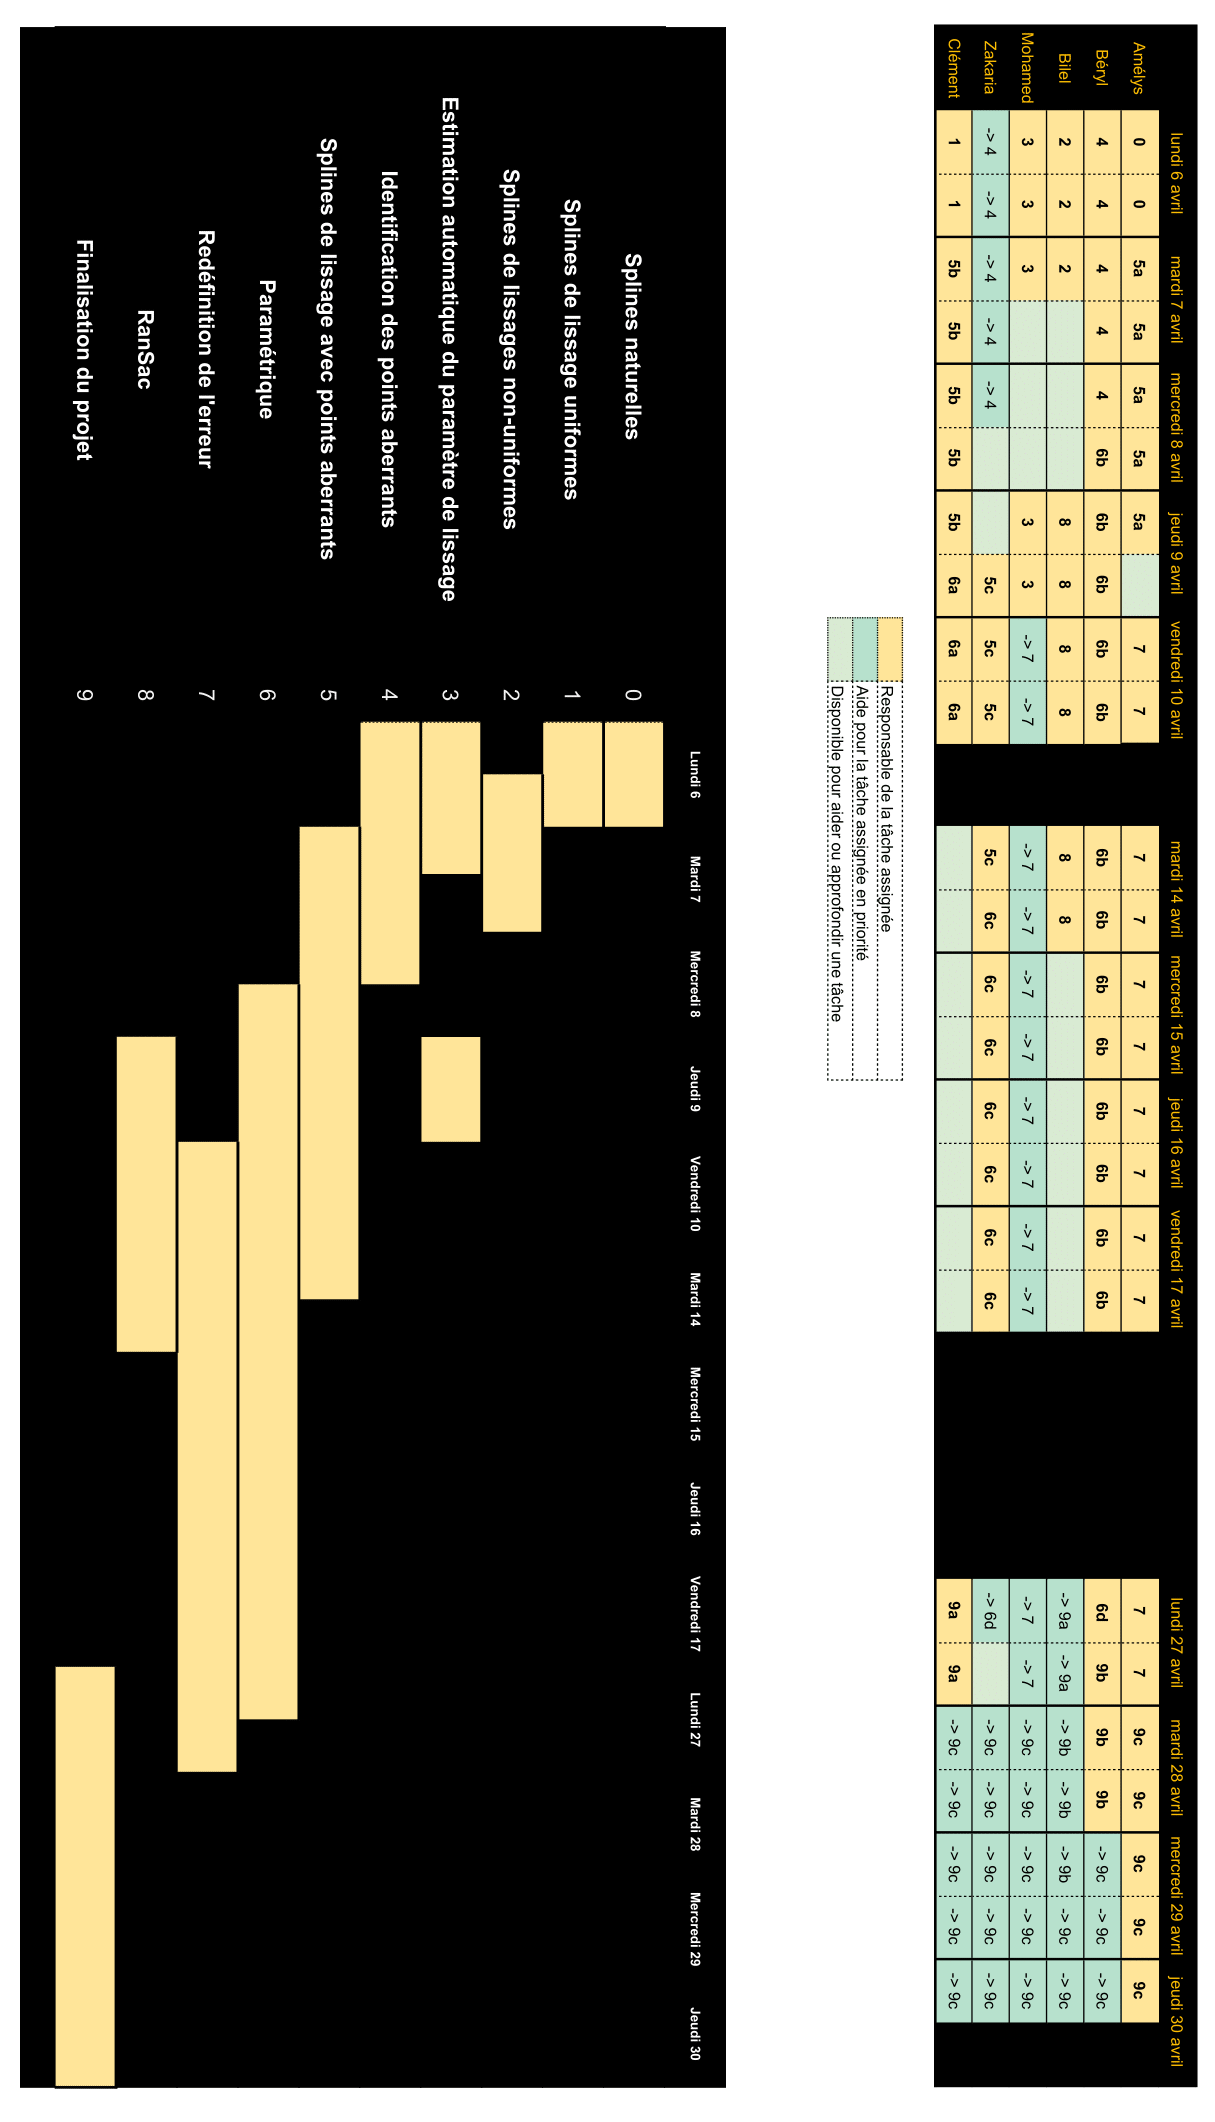
\includegraphics[width=14cm]{p3.png} 
\end{center}
\caption{Diagramme de Gantt simplifié et répartition des tâches}
\label{DiagS}
\end{figure}


\end{document} %Ne rien ecrire apres